% plot-cot-x2.tex — y = cot(x^2), via pgfplots.
% cot(t) = cos(t)/sin(t); pgfplots trig takes degrees, so feed deg(x^2).
\documentclass[border=8pt]{standalone}
\usepackage{pgfplots}
\pgfplotsset{compat=1.18}
\begin{document}
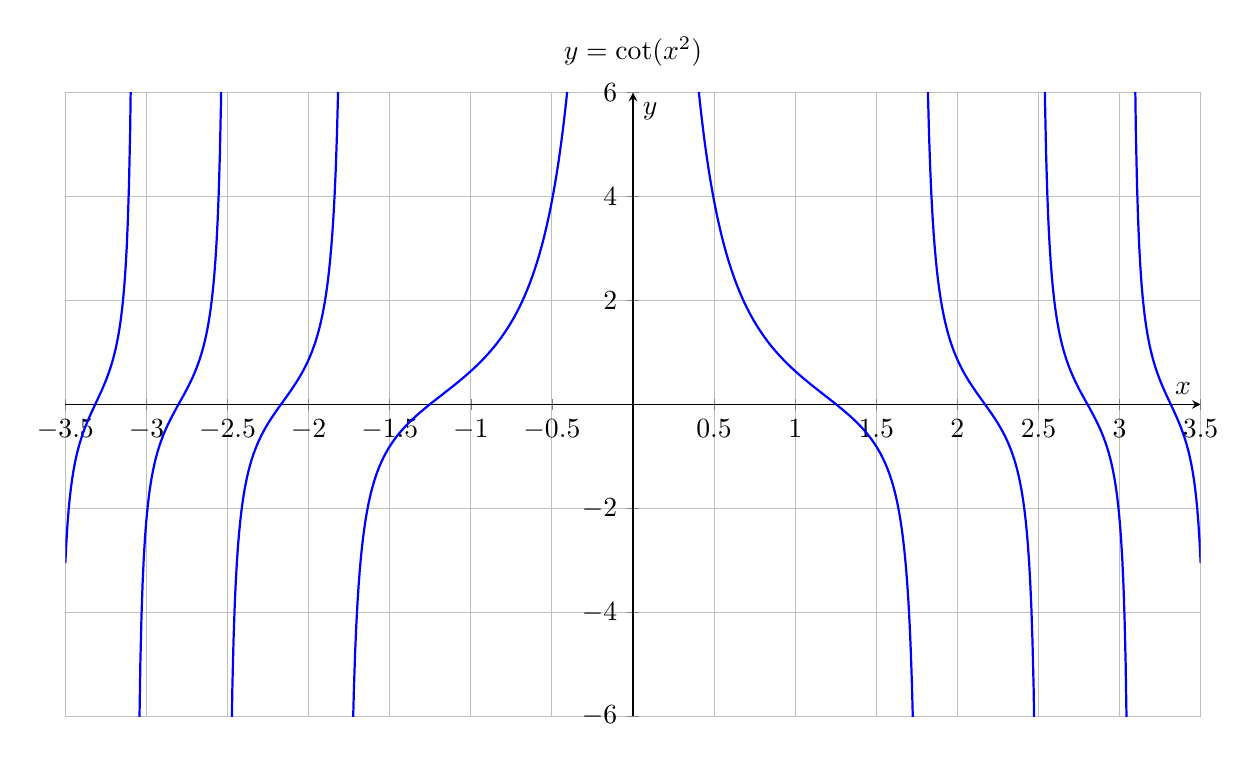
\begin{tikzpicture}
  \begin{axis}[
      axis lines=middle, xlabel=$x$, ylabel=$y$,
      title={$y=\cot(x^2)$},
      domain=-3.5:3.5, samples=1000,
      restrict y to domain=-12:12, ymin=-6, ymax=6,
      unbounded coords=jump, grid=both,
      width=16cm, height=9.5cm]
    \addplot[blue, thick, no marks] {cos(deg(x^2))/sin(deg(x^2))};
  \end{axis}
\end{tikzpicture}
\end{document}
